\subsection{Experimental Series 2. Cloud Task Scheduling}\label{sec:cloudsim_exp}
\subsubsection{Experimental Settings and Protocol}\label{sec:cloud_protocol}
The primary cloud comparison uses 50 heterogeneous VMs and $N=100,200,\ldots,1000$ independent tasks. Workloads are uniform integers from $[1000,20000]$ MI and default processing rates are uniform integers from $[500,2000]$ MIPS. Seeds 43--72 define 30 paired scenarios per scale, giving 300 primary blocks. Nine additional scales, $N=2000,3000,\ldots,10000$, extend the comparison. Separate task and VM random streams generate each scenario, with VM pools shared across scales within a seed. All search fitness is analytical.

Every available VM is reserved from time zero through the analytical makespan and billed continuously at its synthetic rate. Parameters are $r_{\mathrm{min}}=0.05$, $r_{\mathrm{max}}=0.20$ units per second and $\epsilon_\nu=1$ MIPS. The energy proxy retains $P^{\mathrm{max}}=250$ W, $\eta_P=0.6$, $\gamma=3$, and 3600 seconds per hour. All fixed-reference floors are $10^{-9}$ in the corresponding units and are inactive in the saved scenarios. Nominal weights are $(0.25,0.25,0.25,0.25)$, giving effective weights $(0.50,0.25,0.25)$ under Eq.~\eqref{eq:cost}. Local admissibility tolerance is $10^{-12}$.

LSCBO, adapted CBO, PSO, GWO, WOA, and adapted AOA use 100 uniformly random population members without a deterministic injected member. The recorded iteration setting is 100 and the nominal candidate allowance is $B=10000$. Termination follows evaluation accounting, not 100 required full sweeps. The population and primary scale settings are inspired by ERTH~\cite{Qin2024}; its cost expression, normalization, algorithm, and results are not reproduced. Greedy-LPT supplies the shared fixed normalization references, assigning tasks in descending workload order to the earliest projected finish, with original-index and smallest-VM-index tie breaking. It is not injected into the random populations or displayed as a population competitor. The released main CSV retains 3420 population-method rows and 570 reference-only rows; these reference records support normalization and audit.

The implemented CBO and L\'{e}vy parameters are retained. Cloud coordinates span $[0,1]$, with the $10^{-10}$ L\'{e}vy safeguard. PSO uses $w=0.9\rightarrow0.4$, $c_1=c_2=2$, initial velocity $0.1\mathcal N(0,1)$, and clipping to $[-0.2,0.2]$. GWO and WOA use $a=2\rightarrow0$; WOA has spiral coefficient 1 and branch probability 0.5. Adapted AOA uses $\alpha=5$, $\mu=0.499$, and MOA from 0.2 to 1. Cloud random streams use \texttt{java.util.Random}, derived from scenario, experiment, variant, and profile identifiers.

LSCBO reserves 600 core candidates and 9400 pair trials, with 400 trials per local round. Initialization consumes 100 core evaluations and core proposals consume 500. Other population comparators use all 10000 candidates in their continuous core. One local-entry reevaluation makes 10001 internal LSCBO scoring calls, or 10002 including the common reference evaluation. At most $\lceil9400/400\rceil=24$ local rounds can commit an exchange, touching at most 48 distinct tasks. The retained archived local sampler and decoder are unchanged by the cost revision.

The new analytical dataset contains 7050 rows: 3990 main rows over 19 scales, 2250 weight rows, and 810 capacity rows. Figures 6 and 7 use only the 2100 primary main rows. Python independently recomputes all four criteria and fitness from every stored assignment and scenario. The primary 2100 rows reproduce the selected-model screening results exactly at stored precision. Main uncertainty uses 30 complete seed clusters, 50000 percentile-bootstrap resamples, and PCG64 seed 20260912. The seed is the resampling unit; scales are retained within each cluster.

\textbf{Exploratory selection and additional-seed confirmation.}
Nine cost candidates were screened in two exploratory stages using seeds 43--72, with optimization repeated under each native definition. The continuous fixed-fleet reservation formula was selected by its mean paired cost advantage against its closest population comparator, PSO. The model and comparator were fixed before testing seeds 103--132. The selected model's mean paired reduction against PSO is 25.1840\% on the screening seeds and 25.6809\% on the new seeds; the latter 95\% seed-cluster interval is 24.6229\%--26.6663\%, with 300/0/0 wins/ties/losses and the lowest mean cost at all ten scales. Confirmation uses 30000 bootstrap resamples with seed 20261011. The main tables reuse screening seeds, so the confirmation supports the selected cost comparison rather than independently validating every main-table claim.

On those same additional instances, the completion-time control is optimized separately. Scoring the new reservation-optimized LSCBO assignments with the old completion-time cost gives values 1.1079\% higher on average than that control, with a 95\% seed-cluster interval of 0.9969\%--1.2258\%. The larger reservation-cost separation therefore reflects the changed charging policy and scalar preference, not an improvement of the earlier cost metric.

\begin{table}[htbp]\centering\small
\caption{Cold-start configurations and internal scoring calls. The shared reference evaluation is additional.}\label{tab:configuration_map}
\setlength{\tabcolsep}{3pt}
\begin{tabular}{lrrrr}
\toprule Method & Core & Pair trials & Internal calls & Population\\
\midrule LSCBO & 600 & 9400 & 10001 & 100\\
Adapted CBO & 10000 & 0 & 10000 & 100\\
PSO & 10000 & 0 & 10000 & 100\\
GWO & 10000 & 0 & 10000 & 100\\
WOA & 10000 & 0 & 10000 & 100\\
Adapted AOA & 10000 & 0 & 10000 & 100\\
\bottomrule\end{tabular}
\par\smallskip{\footnotesize Sensitivity uses the same complete scheduler and core/local split. Normalization adds one shared reference call per instance outside the population allowance.\par}
\end{table}\FloatBarrier
\subsubsection{Main Comparison}
LSCBO has the lowest mean $F$ among the six population methods at all ten primary task scales. Its overall mean is 19.953855, compared with 25.704472--31.134720 for the other population methods and 1 for Greedy-LPT. These are scale-mean rankings, not claims of a win in every paired seed. Table~\ref{tab:cloud_main_objective} reports the six population methods. Resampling complete seed clusters gives a 95\% interval of 19.311615--20.616214 for LSCBO's primary mean $F$.
\begin{table*}[!htbp]
\centering\small
\caption{Cold-start mean reference-normalized objective $F$ over 30 paired seeds at each primary task scale (lower is better). Only the six population methods are displayed; reference construction is defined in Section~\ref{sec:cloud_protocol}.}\label{tab:cloud_main_objective}
\resizebox{\textwidth}{!}{%
\begin{tabular}{l c c c c c c}
\toprule
Tasks & LSCBO & CBO & PSO & GWO & WOA & Adapted AOA \\
\midrule
100 & 3.4046 & 4.5759 & 5.2214 & 6.3786 & 5.4342 & 6.3717 \\
200 & 6.5952 & 10.1033 & 10.7299 & 13.1799 & 11.1067 & 13.2568 \\
300 & 9.0984 & 14.6207 & 15.0726 & 17.9760 & 14.7277 & 18.0556 \\
400 & 13.8638 & 21.1788 & 21.0465 & 25.0603 & 21.1661 & 25.0765 \\
500 & 18.3725 & 27.2336 & 25.4814 & 31.1117 & 26.3336 & 31.2172 \\
600 & 20.9774 & 29.1115 & 27.5281 & 32.9948 & 28.2043 & 33.1799 \\
700 & 24.9995 & 33.7967 & 31.4594 & 38.0532 & 33.1611 & 38.1118 \\
800 & 30.4452 & 40.4519 & 36.3089 & 44.7519 & 38.9461 & 44.6780 \\
900 & 34.1787 & 44.7063 & 41.1325 & 49.3416 & 41.0689 & 48.9646 \\
1000 & 37.6033 & 47.9044 & 43.0639 & 52.0647 & 44.6275 & 52.4352 \\
\bottomrule
\end{tabular}
}
\end{table*}
\begin{table*}[!htbp]
\centering\small
\caption{Cold-start LSCBO relative reductions over the shared fixed reference. Negative reductions indicate worse outcomes. Component reductions are ratios of scale-wise means; $F$ reductions are means of paired instance reductions. Parentheses report paired W/T/L counts (30 seeds).}\label{tab:main_improvement}
\resizebox{\textwidth}{!}{%
\begin{tabular}{l c c c c c}
\toprule
Tasks & Makespan & Energy & Cost & $\mathcal{I}$ & $F$ \\
\midrule
100 & \shortstack{-38.8736\%\\(0/0/30)} & \shortstack{-16.7167\%\\(0/0/30)} & \shortstack{-38.7936\%\\(0/0/30)} & \shortstack{-802.0890\%\\(0/0/30)} & \shortstack{-240.4620\%\\(0/0/30)} \\
200 & \shortstack{-40.0549\%\\(0/0/30)} & \shortstack{-11.9073\%\\(0/0/30)} & \shortstack{-40.0203\%\\(0/0/30)} & \shortstack{-1968.8160\%\\(0/0/30)} & \shortstack{-559.5157\%\\(0/0/30)} \\
300 & \shortstack{-42.0570\%\\(0/0/30)} & \shortstack{-11.9373\%\\(0/0/30)} & \shortstack{-41.9791\%\\(0/0/30)} & \shortstack{-2954.5294\%\\(0/0/30)} & \shortstack{-809.8373\%\\(0/0/30)} \\
400 & \shortstack{-45.9823\%\\(0/0/30)} & \shortstack{-13.4877\%\\(0/0/30)} & \shortstack{-46.0063\%\\(0/0/30)} & \shortstack{-4763.1286\%\\(0/0/30)} & \shortstack{-1286.3771\%\\(0/0/30)} \\
500 & \shortstack{-49.1954\%\\(0/0/30)} & \shortstack{-14.9795\%\\(0/0/30)} & \shortstack{-49.1657\%\\(0/0/30)} & \shortstack{-6431.1607\%\\(0/0/30)} & \shortstack{-1737.2532\%\\(0/0/30)} \\
600 & \shortstack{-50.9174\%\\(0/0/30)} & \shortstack{-16.3763\%\\(0/0/30)} & \shortstack{-50.8768\%\\(0/0/30)} & \shortstack{-7663.3794\%\\(0/0/30)} & \shortstack{-1997.7350\%\\(0/0/30)} \\
700 & \shortstack{-54.3047\%\\(0/0/30)} & \shortstack{-17.7835\%\\(0/0/30)} & \shortstack{-54.2718\%\\(0/0/30)} & \shortstack{-9236.8181\%\\(0/0/30)} & \shortstack{-2399.9517\%\\(0/0/30)} \\
800 & \shortstack{-59.0601\%\\(0/0/30)} & \shortstack{-19.6090\%\\(0/0/30)} & \shortstack{-59.1069\%\\(0/0/30)} & \shortstack{-11346.9547\%\\(0/0/30)} & \shortstack{-2944.5152\%\\(0/0/30)} \\
900 & \shortstack{-58.9449\%\\(0/0/30)} & \shortstack{-19.7759\%\\(0/0/30)} & \shortstack{-58.9044\%\\(0/0/30)} & \shortstack{-12802.3247\%\\(0/0/30)} & \shortstack{-3317.8728\%\\(0/0/30)} \\
1000 & \shortstack{-61.9330\%\\(0/0/30)} & \shortstack{-21.4052\%\\(0/0/30)} & \shortstack{-61.8518\%\\(0/0/30)} & \shortstack{-14239.4761\%\\(0/0/30)} & \shortstack{-3660.3349\%\\(0/0/30)} \\
\bottomrule
\end{tabular}
}
\end{table*}

\FloatBarrier
All four LSCBO criteria are higher than Greedy-LPT in every one of the 300 primary instances. Its mean paired reservation-cost increase over the reference is 50.0934\%. Reservation cost and makespan have identical paired relative changes because the fixed fleet-price sum cancels. The negative reductions in Table~\ref{tab:main_improvement} are therefore regressions, and the incumbent-relative guard does not establish reference-relative non-regression.

Among the population methods, LSCBO has the lowest mean reservation cost at every primary scale. Its mean paired cost reduction against the fixed PSO comparator is 25.1840\%, with 298/0/2 wins/ties/losses on the main seeds. Figure~\ref{fig:cloud_large_scale_costs}(c) shows this separation in absolute synthetic units. For a given seed, Cost is exactly a constant multiple of makespan. Since fleet prices vary by seed, aggregated cost means are price-weighted horizon means; an average curve need not be one globally fixed multiple of the makespan curve. The cost panel is a policy-specific financial interpretation of batch duration, not additional independent optimization evidence.

Figure~\ref{fig:cloud_small_scale_costs} shows mean normalized objectives on a logarithmic axis. Figure~\ref{fig:cloud_large_scale_costs} shows absolute component means. The curves and comparison tables display the population methods. Shared normalization references are specified in Section~\ref{sec:cloud_protocol} and retained in the released raw records. There is no cost inset, smoothing, self-relative reference line, or vertical offset.
\begin{figure*}[htbp]\centering
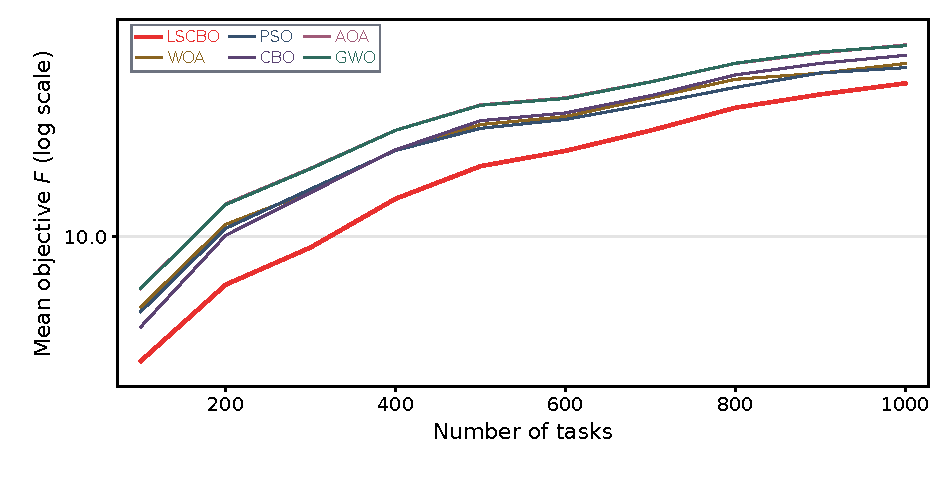
\includegraphics[width=\textwidth]{图/Fig6.pdf}
\caption{Cold-start comparison at 100--1000 tasks: 100 random population members, a 10000-candidate allowance, 50 VMs, and 30 paired seeds per scale. Mean normalized $F$ for six population methods is shown on a logarithmic axis under batch reservation charging. Shared reference normalization is defined in Section~\ref{sec:cloud_protocol}.}\label{fig:cloud_small_scale_costs}
\end{figure*}
\begin{figure*}[htbp]\centering
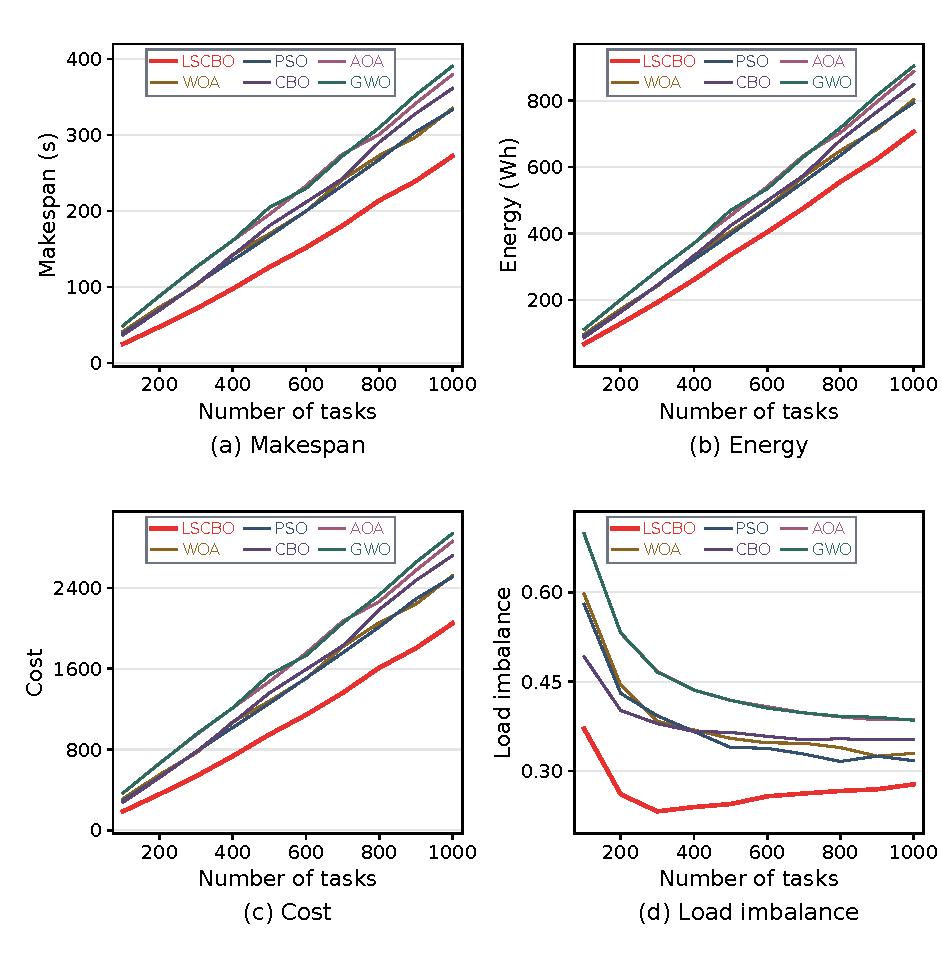
\includegraphics[width=\textwidth]{图/Fig7.pdf}
\caption{Cold-start absolute analytical means over 30 paired seeds per scale: (a) makespan, (b) energy, (c) batch reservation cost, and (d) load imbalance. Every VM is charged from zero until common release at batch completion, at synthetic continuous rates. Normalized cost equals normalized makespan within each instance. Each method has the same color, solid line, and width in all panels and the legend. Shared reference normalization is defined in Section~\ref{sec:cloud_protocol}; the underlying reference records accompany the raw data.}\label{fig:cloud_large_scale_costs}
\end{figure*}\FloatBarrier
\begin{table}[!htbp]
\centering\small
\setlength{\tabcolsep}{4pt}
\caption{Cold-start absolute analytical outcomes for LSCBO at all ten primary task scales. Each cell gives the mean on the first line and sample standard deviation in parentheses below, over 30 paired seeds (divisor 29). Batch reservation cost uses synthetic units and charges the entire fixed VM fleet through makespan; $\mathcal{I}$ and $F$ are dimensionless.}\label{tab:main_scale_dispersion}
\begin{tabular}{l c c c c c}
\toprule
Tasks & $H_{\max}$ (s) & $E$ (Wh) & $C$ (units) & $\mathcal{I}$ & $F$ \\
\midrule
100 & \shortstack{24.803\\(2.915)} & \shortstack{67.395\\(6.494)} & \shortstack{186.775\\(19.354)} & \shortstack{0.37109\\(0.05427)} & \shortstack{3.405\\(0.755)} \\
200 & \shortstack{47.435\\(4.038)} & \shortstack{128.852\\(9.501)} & \shortstack{357.246\\(24.197)} & \shortstack{0.26104\\(0.04185)} & \shortstack{6.595\\(1.821)} \\
300 & \shortstack{71.165\\(5.656)} & \shortstack{192.498\\(13.139)} & \shortstack{535.959\\(31.814)} & \shortstack{0.23232\\(0.02779)} & \shortstack{9.098\\(2.146)} \\
400 & \shortstack{97.459\\(5.659)} & \shortstack{261.210\\(14.676)} & \shortstack{734.494\\(33.540)} & \shortstack{0.23959\\(0.02619)} & \shortstack{13.864\\(3.488)} \\
500 & \shortstack{125.993\\(9.320)} & \shortstack{335.354\\(19.682)} & \shortstack{949.328\\(57.574)} & \shortstack{0.24462\\(0.02175)} & \shortstack{18.373\\(5.753)} \\
600 & \shortstack{151.732\\(11.150)} & \shortstack{404.373\\(24.897)} & \shortstack{1143.133\\(66.586)} & \shortstack{0.25760\\(0.02685)} & \shortstack{20.977\\(3.963)} \\
700 & \shortstack{180.703\\(12.185)} & \shortstack{476.994\\(28.358)} & \shortstack{1361.220\\(64.676)} & \shortstack{0.26233\\(0.02528)} & \shortstack{25.000\\(3.893)} \\
800 & \shortstack{213.712\\(15.652)} & \shortstack{556.142\\(34.786)} & \shortstack{1610.678\\(104.967)} & \shortstack{0.26659\\(0.02458)} & \shortstack{30.445\\(5.187)} \\
900 & \shortstack{239.444\\(17.131)} & \shortstack{624.647\\(39.423)} & \shortstack{1803.612\\(95.282)} & \shortstack{0.26939\\(0.02386)} & \shortstack{34.179\\(6.169)} \\
1000 & \shortstack{272.157\\(22.448)} & \shortstack{706.486\\(46.948)} & \shortstack{2049.752\\(132.202)} & \shortstack{0.27769\\(0.02487)} & \shortstack{37.603\\(5.824)} \\
\bottomrule
\end{tabular}
\end{table}
\FloatBarrier
The nine external scales retain the same cost policy and candidate allowance. WOA overtakes LSCBO at $N\in\{4000, 5000, 6000, 7000, 8000, 9000, 10000\}$, lowering scale-wise mean $F$ by 0.50--8.34\% relative to LSCBO. LSCBO retains a lower or equal mean than WOA at $N\in\{2000, 3000\}$. The released CSV contains all 19 scales. The large-scale crossover limits the primary ranking.
\subsubsection{Direct Greedy-LPT Refinement}\label{sec:direct_pair}
The direct-refinement diagnostic uses the same 300 primary scenarios, equal nominal weights, 50 VMs, and batch reservation charging. A separately compiled instrumented diagnostic reproduces LSCBO's five stored outcome metrics in all 300 blocks. The two displayed controls explicitly start from Greedy-LPT and run 9400 or 10000 Pareto-safe pair trials. Their total scoring counts, including reference and local-entry scoring, are 9402 and 10002. This initialization is different from the primary random-start protocol.

The mean objectives are 0.974373 and 0.973684 for the 9400- and 10000-trial controls. Their lower/tied/higher counts against Greedy-LPT are 300/0/0 and 300/0/0. The 10000-trial versus 9400-trial objective counts are 190/110/0. The guard protects the current incumbent's makespan, energy, cost, and imbalance, with the cost constraint mathematically redundant under common release. Changing the final partial round can alter the chosen exchange, so an objective improvement need not dominate every component across separately terminated runs.

Timing uses an Intel Core i7-14650HX Windows 11 machine, 24 logical CPUs, about 32 GB RAM, and Microsoft OpenJDK 21.0.7. One application thread and Serial GC use a 512 MB initial and 2 GB maximum heap. After metric reproduction and two complete warm-up cycles, five repetitions rotate method order. Reported times are means of within-block medians and include reference construction, normalization, and search, but exclude scenario generation, hashing, and CSV output. The analytical main and sensitivity jobs finish before timing begins. Frequency and affinity are not fixed; the measurements are descriptive.
\begin{table}[!htbp]\centering\small
\setlength{\tabcolsep}{4pt}
\caption{Direct Greedy-initialized pair controls under batch reservation charging on 300 paired scenarios. Calls include reference and local-entry scoring; times are means of within-block medians over five warmed repetitions.}\label{tab:direct_pair}
\begin{tabular}{p{.36\textwidth}rrrr}\toprule
Method & \shortstack{Actual\\calls} & Mean $F$ & \shortstack{Mean accepted\\exchanges} & \shortstack{Time\\(ms)}\\\midrule
Greedy + pair search, 9400 trials & 9402 & 0.974373 & 16.62 & 32.31 \\
Greedy + pair search, 10000 trials & 10002 & 0.973684 & 17.34 & 34.40 \\
\bottomrule\end{tabular}\end{table}

\FloatBarrier
\subsubsection{Weight Sensitivity}\label{sec:weight_sensitivity}
Five nominal profiles are evaluated at $N\in\{100,300,500,800,1000\}$ with 30 seeds, 50 VMs, and the same 10000-candidate allowance. The profiles are equal weights and makespan-, energy-, cost-, and balance-priority weights; the named priority receives 0.55 and each other criterion 0.15. LSCBO and adapted CBO produce 1500 optimized records; 750 separate reference-only records support normalization, giving 2250 released rows.

The LSCBO means are 19.7924, 12.6171, 12.4294, 12.6148, 41.7855 in that profile order. Each profile's mean exceeds the fixed reference of 1. Absolute $F$ values from different weights express different scalar preferences and should not be ranked as if one objective were unchanged. Table~\ref{tab:weight_scale_details} reports every scale separately.

Since normalized cost equals normalized makespan, both nominal makespan and cost priorities reduce to effective weights $(0.70,0.15,0.15)$ for makespan, energy, and imbalance. Their stored outcomes differ because the retained implementation derives random streams from profile identifiers, and floating-point evaluation can also differ. These results are not evidence for distinct time and cost preferences. The other effective profiles are $(0.30,0.55,0.15)$ for energy and $(0.30,0.15,0.55)$ for imbalance. Profile sensitivity remains conditional on these preferences and does not identify a universal optimum or a Pareto front~\cite{MarlerArora2010}.
\begin{table*}[!htbp]
\centering\small
\caption{Cold-start sensitivity by task scale: LSCBO objective dispersion and paired reductions over the shared fixed reference.}\label{tab:weight_scale_details}
\resizebox{\textwidth}{!}{%
\begin{tabular}{l c c c c c}
\toprule
Priority & Tasks & Mean $F$ $\pm$ SD & $F$ reduction (\%) & $\mathcal{I}$ reduction (\%) & W/T/L \\
\midrule
Equal & 100 & 3.436255 $\pm$ 0.649934 & -243.6255 & -876.3666 & 0/0/30 \\
Equal & 300 & 9.177249 $\pm$ 2.097877 & -817.7249 & -3175.1270 & 0/0/30 \\
Equal & 500 & 18.790173 $\pm$ 5.682190 & -1779.0173 & -6997.1414 & 0/0/30 \\
Equal & 800 & 30.108801 $\pm$ 4.947311 & -2910.8801 & -11511.6025 & 0/0/30 \\
Equal & 1000 & 37.449336 $\pm$ 5.367060 & -3644.9336 & -14436.3790 & 0/0/30 \\
Makespan & 100 & 2.755092 $\pm$ 0.414323 & -175.5092 & -949.2229 & 0/0/30 \\
Makespan & 300 & 6.174497 $\pm$ 1.303689 & -517.4497 & -3240.3063 & 0/0/30 \\
Makespan & 500 & 12.057427 $\pm$ 3.482799 & -1105.7427 & -7118.6393 & 0/0/30 \\
Makespan & 800 & 18.909402 $\pm$ 3.149117 & -1790.9402 & -11657.6801 & 0/0/30 \\
Makespan & 1000 & 23.188838 $\pm$ 3.173381 & -2218.8838 & -14482.0037 & 0/0/30 \\
Energy & 100 & 2.606991 $\pm$ 0.375961 & -160.6991 & -921.5759 & 0/0/30 \\
Energy & 300 & 6.009445 $\pm$ 1.300605 & -500.9445 & -3213.0211 & 0/0/30 \\
Energy & 500 & 11.867451 $\pm$ 3.599432 & -1086.7451 & -7083.0945 & 0/0/30 \\
Energy & 800 & 18.673201 $\pm$ 2.953601 & -1767.3201 & -11603.0906 & 0/0/30 \\
Energy & 1000 & 22.990036 $\pm$ 3.202573 & -2199.0036 & -14456.3219 & 0/0/30 \\
Cost & 100 & 2.754723 $\pm$ 0.393049 & -175.4723 & -954.3222 & 0/0/30 \\
Cost & 300 & 6.175898 $\pm$ 1.247661 & -517.5898 & -3242.0206 & 0/0/30 \\
Cost & 500 & 12.133824 $\pm$ 3.657125 & -1113.3824 & -7172.9339 & 0/0/30 \\
Cost & 800 & 18.874548 $\pm$ 3.118332 & -1787.4548 & -11633.2789 & 0/0/30 \\
Cost & 1000 & 23.135242 $\pm$ 3.177319 & -2213.5242 & -14449.9269 & 0/0/30 \\
Balance & 100 & 5.777895 $\pm$ 1.501541 & -477.7895 & -842.3375 & 0/0/30 \\
Balance & 300 & 18.355800 $\pm$ 4.318211 & -1735.5800 & -3129.4018 & 0/0/30 \\
Balance & 500 & 39.729406 $\pm$ 13.032062 & -3872.9406 & -7009.1862 & 0/0/30 \\
Balance & 800 & 64.811614 $\pm$ 11.168877 & -6381.1614 & -11565.3267 & 0/0/30 \\
Balance & 1000 & 80.252641 $\pm$ 11.887667 & -7925.2641 & -14369.5442 & 0/0/30 \\
\bottomrule
\multicolumn{6}{p{.97\textwidth}}{\footnotesize Each row uses 30 paired seeds and 50 VMs. Reductions are means of instance-wise percentages; negative values indicate regressions. The shared fixed reference has $F=1.000000\pm0.000000$. W/T/L uses an absolute $10^{-8}$ tie threshold on $F$. Equal weights are (0.25,0.25,0.25,0.25); a priority uses weight 0.55 and 0.15 for the other criteria.}\\
\end{tabular}
}
\end{table*}

\FloatBarrier
\subsubsection{VM Heterogeneity}\label{sec:vm_heterogeneity}
Processing rates are sampled as uniform integers from $[1333,2000]$, $[400,2000]$, and $[100,2000]$ MIPS, labeled approximately 1.5:1, 5:1, and 20:1. Each profile uses $N\in\{500,1000,2000\}$, 30 seeds, 50 VMs, and nominal equal weights. The 2000-task cell extends beyond the primary main-comparison range. Each capacity profile also changes the capacity-normalized price mapping; the comparison does not isolate a causal capacity effect.

The LSCBO mean objectives are 24.189983, 50.219427, 53.619678 for the 1.5:1, 5:1, and 20:1 profiles, respectively. All exceed the corresponding Greedy-LPT reference. Table~\ref{tab:heterogeneity_scale_details} provides the complete scale/profile values. Changing fleet prices rescales absolute Cost, but within a fixed scenario its normalized ratio remains equal to the makespan ratio. Thus a larger absolute bill across profiles is not by itself evidence of a worse independent cost objective.
\begin{table*}[!htbp]
\centering\small
\caption{Cold-start sensitivity by task scale: LSCBO objective dispersion and paired reductions over the shared fixed reference.}\label{tab:heterogeneity_scale_details}
\resizebox{\textwidth}{!}{%
\begin{tabular}{l c c c c c}
\toprule
Capacity ratio & Tasks & Mean $F$ $\pm$ SD & $F$ reduction (\%) & $\mathcal{I}$ reduction (\%) & W/T/L \\
\midrule
1.5:1 & 500 & 10.454794 $\pm$ 3.966480 & -945.4794 & -3734.8643 & 0/0/30 \\
1.5:1 & 1000 & 21.415776 $\pm$ 4.519804 & -2041.5776 & -8119.6961 & 0/0/30 \\
1.5:1 & 2000 & 40.699381 $\pm$ 6.188546 & -3969.9381 & -15836.6628 & 0/0/30 \\
5:1 & 500 & 18.582451 $\pm$ 4.125177 & -1758.2451 & -6886.8083 & 0/0/30 \\
5:1 & 1000 & 42.506956 $\pm$ 6.672730 & -4150.6956 & -16409.8914 & 0/0/30 \\
5:1 & 2000 & 89.568875 $\pm$ 12.038847 & -8856.8875 & -35190.3535 & 0/0/30 \\
20:1 & 500 & 22.176768 $\pm$ 5.920106 & -2117.6768 & -8058.3183 & 0/0/30 \\
20:1 & 1000 & 45.268714 $\pm$ 11.809057 & -4426.8714 & -17123.1008 & 0/0/30 \\
20:1 & 2000 & 93.413551 $\pm$ 28.442079 & -9241.3551 & -36171.0771 & 0/0/30 \\
\bottomrule
\multicolumn{6}{p{.97\textwidth}}{\footnotesize Each row uses 30 paired seeds and 50 VMs. Reductions are means of instance-wise percentages; negative values indicate regressions. The shared fixed reference has $F=1.000000\pm0.000000$. W/T/L uses an absolute $10^{-8}$ tie threshold on $F$. Capacity profiles change both speeds and their capacity-dependent price mapping.}\\
\end{tabular}
}
\end{table*}

\begin{figure*}[htbp]\centering
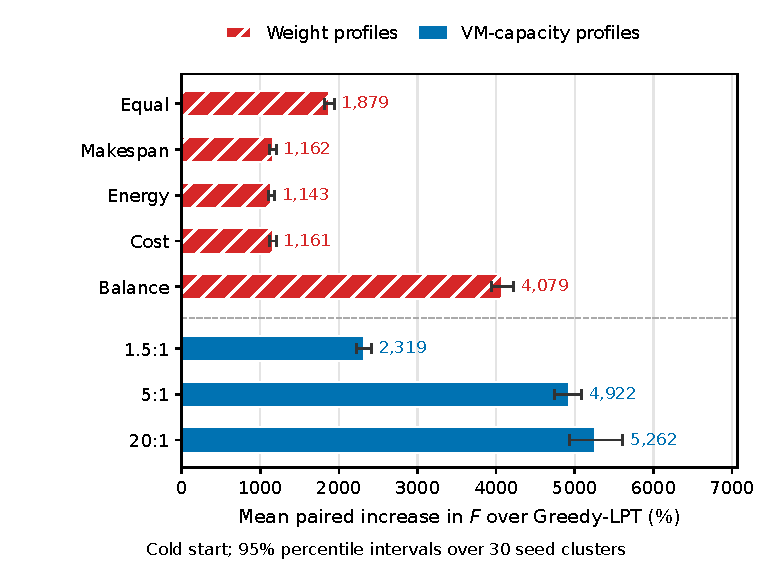
\includegraphics[width=\textwidth]{图/Fig8.pdf}
\caption{Cold-start sensitivity under batch reservation charging. Bars show mean paired increases over the shared fixed reference objective, $100(F/F_g-1)$; lower is better. Five weight profiles retain five scales each, and three VM-capacity profiles retain three scales each. Intervals are 95\% seed-cluster percentile intervals from 30 clusters and 50000 resamples (PCG64 seed 20260912). Nominal makespan and cost priorities have identical effective weights but use different profile-derived random streams. The dashed separator distinguishes the two profile families. These are objective increases, not monetary savings.}\label{fig:profile_sensitivity}
\end{figure*}\FloatBarrier
\subsubsection{Descriptive Runtime Analysis}\label{sec:runtime_descriptive}
The primary analytical logs give LSCBO scale-wise median runtimes from 19.0--111.0 ms. Table~\ref{tab:runtime_descriptive} reports LSCBO median and interquartile ranges. These jobs use eight main workers, while a six-worker sensitivity job runs concurrently. They are not controlled speed comparisons. The warmed single-thread direct experiment provides a separate, still platform-specific timing description. Stored quality observations are not multiplied by timing repetitions.
\begin{table}[!htbp]
\centering\small
\caption{Cold-start LSCBO runtime (ms), median [first quartile, third quartile] over 30 seeds. Concurrent logs are descriptive, not controlled timing benchmarks.}\label{tab:runtime_descriptive}
\begin{tabular}{l c}
\toprule
Tasks & LSCBO with pair search \\
\midrule
100 & 19.0 [17.00, 21.75] \\
200 & 51.0 [23.25, 56.00] \\
300 & 63.0 [60.25, 70.00] \\
400 & 72.5 [70.00, 79.00] \\
500 & 86.0 [81.00, 95.00] \\
600 & 94.0 [89.00, 105.50] \\
700 & 104.5 [98.00, 111.00] \\
800 & 111.0 [105.25, 117.00] \\
900 & 79.0 [75.00, 81.75] \\
1000 & 86.0 [82.25, 90.75] \\
\bottomrule
\end{tabular}
\end{table}

\FloatBarrier
